\documentclass{article}
\usepackage{amsmath,amssymb,amstext,amsfonts}
\usepackage{color}
\usepackage{url}
\usepackage{algorithmic,algorithm}	
\usepackage{listings} 
	% Python style for highlighting
	\newcommand\pythonstyle{\lstset{
	language=Python,
	basicstyle=\ttm,
	otherkeywords={self},             % Add keywords here
	keywordstyle=\ttb\color{deepblue},
	emph={MyClass,__init__},          % Custom highlighting
	emphstyle=\ttb\color{deepred},    % Custom highlighting style
	stringstyle=\color{deepgreen},
	frame=tb,                         % Any extra options here
	showstringspaces=false            % 
	}}
	% Python environment  % use \begin{python} \end{python}
	\lstnewenvironment{python}[1][]
	{
	\pythonstyle
	\lstset{#1}
	}
	{}
	% Python for external files
	\newcommand\pythonexternal[2][]{{
	\pythonstyle
	\lstinputlisting[#1]{#2}}}
	% Python for inline
	\newcommand\pythoninline[1]{{\pythonstyle\lstinline!#1!}}

\usepackage[pdftex]{graphicx}
  \graphicspath{{figures/}}
  \DeclareGraphicsExtensions{.pdf,.jpg,.jpeg,.png}

\newcommand{\norm}[1]{\left\|{#1}\right\|}
\newcommand{\abs}[1]{\left|{#1}\right|}
\newcommand{\defeq}{\stackrel{\triangle}{=}}

\newcommand{\TODO}[1]{{\color{red}#1}}


\title{\LARGE \bf
B-Splines for Robotic Applications
}
\date{Updated: \today}

\author{Randal~W.~Beard \\ Brigham Young University}

\begin{document}

\maketitle

\begin{abstract}
These notes provide an overview of b-splines and their applications to robotics.  In particular, we have in mind applications to path planning for aerial vehicles, model predictive control, and fixed-lag state estimation.  
\end{abstract}

%---------------------------------------------------------------
\section{Motivation}

The objective of these notes is to explore spline methods for robotic applications. In general, the position of a robot in Euclidian space can be described by a time parametrized trajectory $\mathbf{p}(t)\in\mathbb{R}^3$, $t\in[a,b]$.  The time parametrized trajectory can be parameterized using a weighted sum of basic function as
\[
\mathbf{p}(t) = \sum_{j=0}^{n-1} \mathbf{c}_j \phi_j(t),
\]
where $\mathbf{c}_j\in\mathbb{R}^3$, and $\phi_j(t)$ are a set of basis functions.  For example, the basis functions could be the set of polynomial power function $\phi_j(t) = t^j/j!$, or the set of sinusoidal function $\phi_j(t) = \sin(\frac{2\pi j}{n}t)$.  The disadvantage of both the polynomial power functions and sinusoidal functions is that the basis functions are defined for all $t\in[a,b]$ and so each control points $\mathbb{c}_j$ influences the entire trajectory.  Another disadvantage is that a large number of basis functions may be required to represent complicated trajectories.  

In these notes, we will use b-spline basis functions which have a number of very nice properties that we will explore.  In particular, a {\em b-spline} trajectory has the following form
\[
\mathbf{p}(t) = \sum_{j=0}^{n} \mathbf{c}_j B_j^k(t;\mathbf{t}),
\]
where $\mathbf{c}_j\in\mathbb{R}^3$ are the control points,  $\mathbf{t}=(\tau_0, \tau_1, \tau_2, \dots, \tau_T)$ are called the knot points where $i<j \implies \tau_i\leq \tau_j$, and $B_j^k(t;\mathbf{t})$ are the b-spline basis functions of order $k$. The spline trajectories will be defined for $t$ in the span of the knot points, i.e., $t\in[\tau_0, \tau_T]$.  

Section~\ref{sec:b-spline-basis-functions} defines the b-spline basis function $B_j^k(t; \mathbf{t})$ and describes some of their properties that will be useful for path planning.
% overview of other sections

%---------------------------------------------------------------
\section{B-Spline Basis Functions}
\label{sec:b-spline-basis-functions}

The B-spline basis function are defined by the following recursive formula:
\begin{align*}
B_j^0(t; \mathbf{t}) &= \begin{cases} 1 & \text{~if~} \tau_j \leq t \leq \tau_{j+1} \\ 
 									 0 & \text{~otherwise} 
 					   \end{cases} \\	
B_j^k(t; \mathbf{t}) &= \frac{t-\tau_j}{\tau_{j+k}-
\tau_j} B_j^{k-1}(t; \mathbf{t}) + \frac{\tau_{j+k+1}-t}{\tau_{j+k+1}-\tau_{j+1}} B_{j+1}^{k-1}(t; \mathbf{t}).
\end{align*}

%+++++++++++++++++++++++++++++++
\subsection{Zeroth order basis}

If the knot vector is given by
\[
\mathbf{t} = [\tau_0, \tau_1, \tau_2] \defeq [0, 1, 2],
\]
then there are two basis function of order $k=0$ given by
\begin{align*}
B_0^0(t; \mathbf{t}) &= \begin{cases} 1 & \text{~if~} \tau_0 \leq t \leq \tau_1 \\ 
 									 0 & \text{~otherwise} 
 			\end{cases}
\\ 
B_1^0(t; \mathbf{t}) &= \begin{cases} 1 & \text{~if~} \tau_1 \leq t \leq \tau_2 \\ 
 									 0 & \text{~otherwise}
 			\end{cases}
\end{align*}
where $B_0^0(t)$ and $B_0^0(t)$ are shown in Figure~\ref{fig:spline_basis_0}.
\begin{figure}[hbt]
  \centering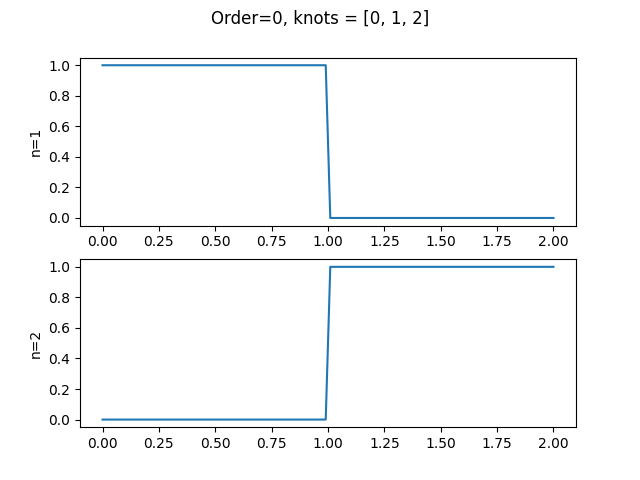
\includegraphics[width=0.5\textwidth]{./figures/spline_basis_0}
  \caption{Zeroth order spline basis}
  \label{fig:spline_basis_0}  
\end{figure}
Additional zeroth order basis function can be defined by expanding the knot vector.

\clearpage


%+++++++++++++++++++++++++++++++
\subsection{First order basis}

If the knot vector is given by
\[
\mathbf{t} = [\tau_0, \tau_1, \tau_2, \tau_3, \tau_4] \defeq [0, 0, 1, 2, 2],
\]
then there are two basis function of order $k=1$ given by
\begin{align*}
B_0^0(t; \mathbf{t}) &= \frac{t-\tau_0}{\tau_1-\tau_0} B_0^0(t;\mathbf{t}) + \frac{\tau_2-t}{\tau_2-\tau_1}B_1^0(t; \mathbf{t}) 
	= \begin{cases} 1-t & \text{~if~} 0 \leq t \leq 1 \\ 
 					0   & \text{~otherwise} 
 	  \end{cases}
\\ 
B_1^1(t; \mathbf{t}) &= \frac{t-\tau_1}{\tau_2-\tau_1} B_1^0(t;\mathbf{t}) + \frac{\tau_3-t}{\tau_3-\tau_2}B_2^0(t; \mathbf{t})
	= \begin{cases} t & \text{~if~} 0 \leq t \leq 1 \\ 
 									2-t & 1 \leq t \leq 2 \\
 									0 & \text{~otherwise}
 					    \end{cases}
\\ 
B_2^1(t; \mathbf{t}) &= \frac{t-\tau_2}{\tau_3-\tau_2} B_2^0(t;\mathbf{t}) + \frac{\tau_4-t}{\tau_4-\tau_3}B_3^0(t; \mathbf{t})
	= \begin{cases} t-1 & \text{~if~} 1 \leq t \leq 2 \\ 
 					0 & \text{~otherwise}
 	  \end{cases}
\end{align*}
where $B_0^1(t; \mathbf{t})$, $B_1^1(t; \mathbf{t})$, and $B_2^1(t; \mathbf{t})$ are shown in Figure~\ref{fig:spline_basis_1}.
\begin{figure}[hbt]
  \centering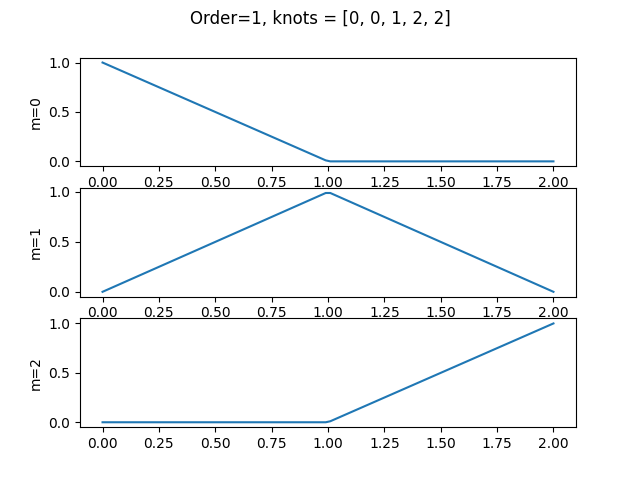
\includegraphics[width=0.7\textwidth]{./figures/spline_basis_1}
  \caption{First order spline basis}
  \label{fig:spline_basis_1}  
\end{figure}
Expanding the knot vector to 
\[
\mathbf{t}' = [\tau_0, \tau_1, \tau_2, \tau_3, \tau_4, \tau_5] \defeq [0, 0, 1, 2, 3, 3],
\]
results in $B_2^1(t; \mathbf{t}')$ looking like $B_1^1(t; \mathbf{t})$ shifted to the right by one, and $B_3^1(t; \mathbf{t}')$ looking like $B_2^1(t; \mathbf{t})$ shifted to the right by one.

\clearpage


%+++++++++++++++++++++++++++++++
\subsection{Second order basis}

\begin{figure}[hbt]
  \centering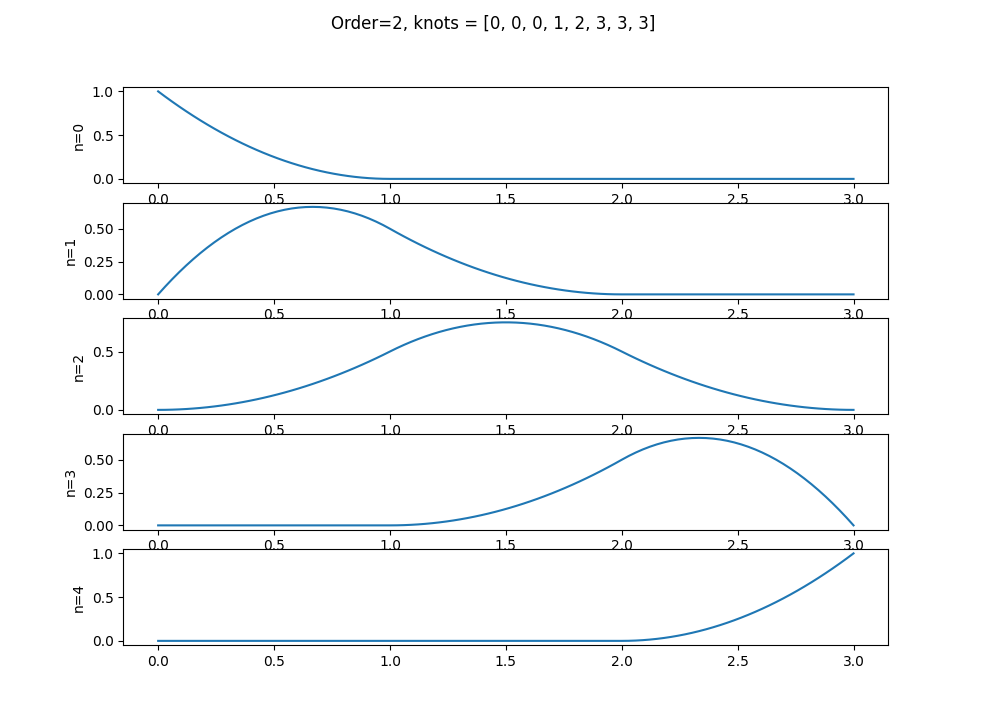
\includegraphics[width=0.5\textwidth]{./figures/spline_basis_2}
  \caption{Second order spline basis}
  \label{fig:spline_basis_2}  
\end{figure}

%+++++++++++++++++++++++++++++++
\subsection{Third order basis}

\begin{figure}[hbt]
  \centering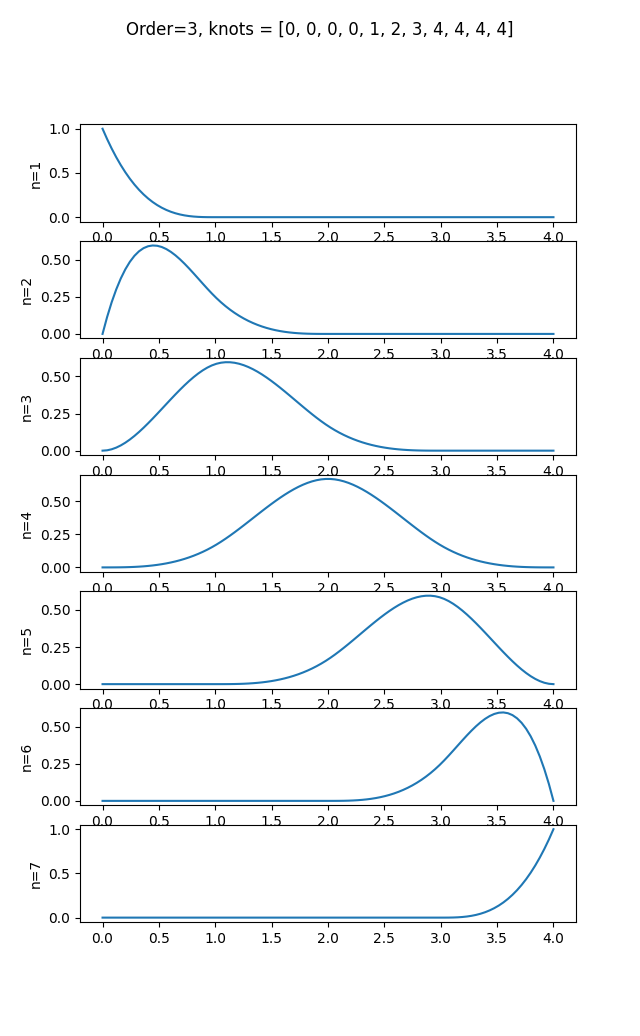
\includegraphics[width=0.5\textwidth]{./figures/spline_basis_3}
  \caption{Third order spline basis}
  \label{fig:spline_basis_3}  
\end{figure}

%+++++++++++++++++++++++++++++++
\subsection{Eigth order basis}

\begin{figure}[hbt]
  \centering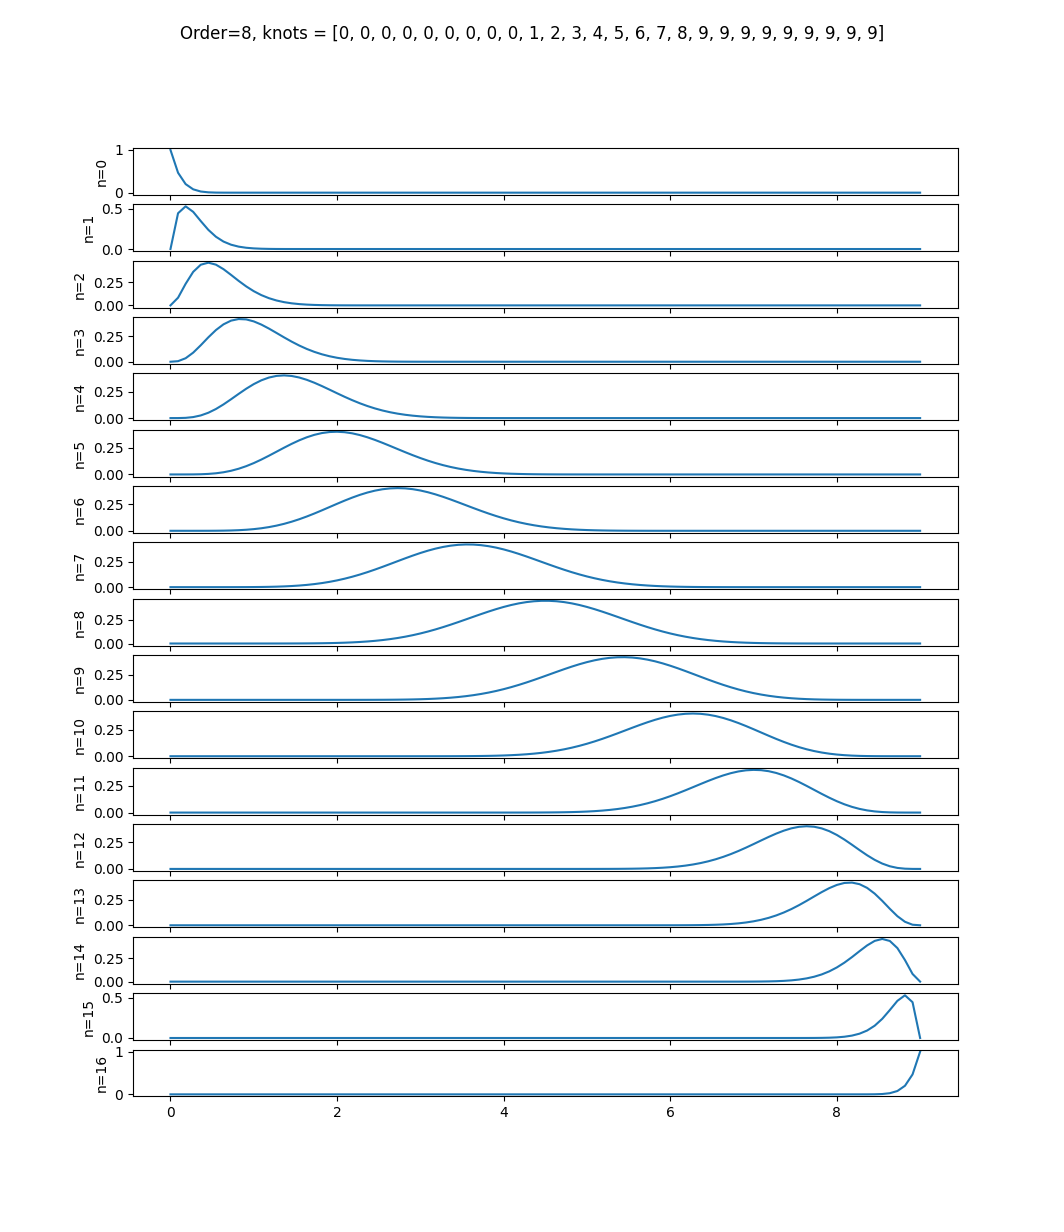
\includegraphics[width=0.5\textwidth]{./figures/spline_basis_8}
  \caption{Eigth order spline basis}
  \label{fig:spline_basis_8}  
\end{figure}


%+++++++++++++++++++++++++++++++
\subsection{Derivative of basis functions}


The general formula for the derivative of the basis functions is~\cite{PieglTiller95}
\[
\frac{d^m}{dt^m}B_j^k(t; \mathbf{t}) = k\left(\frac{\frac{d^{m-1}}{dt^{m-1}}B_j^{k-1}(t; \mathbf{t})}{t_{j+k}-t_j} - \frac{\frac{d^{m-1}}{dt^{m-1}}B_{j+1}^{k-1}(t; \mathbf{t})}{t_{j+k+1}-t_{j+1}} \right).
\]


%---------------------------------------------------------------
\section{B-Spline Trajectories}

If the $k^{th}$-order B-spline curve with knot vector 
\[
\mathbf{t} = \boldsymbol{\tau} = (\tau_0, \tau_1, \dots, \tau_K)
\] 
is given by
\[
\mathbf{C}(t) = \sum_{j=0}^n B_j^k(t;\mathbf{t}) \mathbf{c}_j, 
\]
where $\{\mathbf{c}_j\}_{j=0}^n$ are called the control points.  

For path planning we will construct paths between the initial time $t_0$ and the final time $t_f>t_0$.  We will divide the time interval into $n$ equal segments, and we will always use a knot vector of length 
\[
K=k+(n+1)+k
\]
where $n\geq m+1$, and where
\[
		k_j = \begin{cases}
 				t_0, & 0\leq j \leq m \\
 				t_0 + \frac{(j-m)(t_f-t_0)}{n}, & m+1 \leq j \leq m+n-1 \\
 				t_f, & m+n \leq j \leq 2m + n + 1
 			  \end{cases}
\]
or 
\[
\mathbf{t}_m = (\underbrace{t_0, t_0, \dots, t_0,}_{m+1} t_0+\Delta, t_0+2\Delta, \dots, t_0+(n-1)\Delta, \underbrace{t_f, t_f, \dots, t_f}_{m+1}),
\]
where $n$ is the number of control points, and $\Delta = (t_f-t_0)/n$.  Knot vectors of this form are said to be {\em uniform} knot vectors.

In the rest of these notes, we will use the shorthand notation
\[
B_j^m(t)\equiv B_j^m(t; \mathbf{t}_m).
\]

The knot vector $\mathbf{t}_m$ has $K=2m+n+1$ elements.  A b-spline with knots $\mathbf{t}_m$ requires a total of $N=n+m$ control points, where one control point is needed for each interval for a total of $n$ control points, and the extra $m$ control points are required to allow the extra degrees of freedom.

\subsection{SciPy BSpline library}
The SciPy library has a spline library.  

The following commands will create a cubic spline.
\begin{lstlisting}
	import numpy as np
	from scipy.interpolate import BSpline

    # initial and final time
    t0 = 0
    tf = 5
    order = 3
    knots = np.array([t0, t0, t0, t0,
                     (tf-t0)/3, 2*(tf-t0)/4,
                     tf, tf, tf, tf])
    # num control > num knots - order - 1
    ctrl_pts = np.array([[0, 0, 0],  
                         [0, 1, 0],
                         [0, 0, 1],
                         [0, 1, 1],
                         [1, 1, 0],
                         [1, 1, 1]])
    spl = BSpline(t=knots, c=ctrl_pts, k=order)
    plotSpline(spl)
\end{lstlisting}

Where {\tt plotSpline} is given below.
\begin{lstlisting}
from math import ceil
from scipy.interpolate import BSpline
import matplotlib.pyplot as plt

def plotSpline(spl):
    t0 = spl.t[0]  # first knot is t0
    tf = spl.t[-1]  # last knot is tf
    # number of points in time vector so spacing is 0.01
    N = ceil((tf - t0)/0.01)
    t = np.linspace(t0, tf, N)  # time vector
    position = spl(t)
    # 3D trajectory plot
    fig = plt.figure(1)
    ax = fig.add_subplot(111, projection='3d')
    # plot control points (convert YX(-Z) -> NED)
    ax.plot(spl.c[:, 1], spl.c[:, 0], -spl.c[:, 2],
            '-o', label='control points')
    # plot spline (convert YX(-Z) -> NED)
    ax.plot(position[:, 1], position[:, 0], -position[:, 2],
            'b', label='spline')
    ax.legend()
    ax.set_xlabel('x', fontsize=16, rotation=0)
    ax.set_ylabel('y', fontsize=16, rotation=0)
    ax.set_zlabel('z', fontsize=16, rotation=0)
    #ax.set_xlim3d([-10, 10])
    plt.show()
\end{lstlisting}

The resulting spline is shown in Figure~\ref{fig:example_spline_curve}.
\begin{figure}[hbt]
  \centering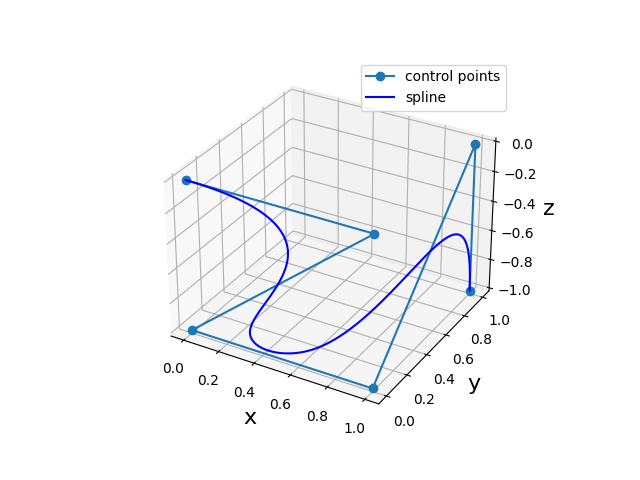
\includegraphics[width=0.5\textwidth]{./figures/example_spline_curve}
  \caption{Example spline curve}
  \label{fig:example_spline_curve}  
\end{figure}

\subsection{Derivatives of b-splines}
The $k^{th}$ derivative of a b-spline is given by
\[
\frac{d^k}{dt^k}\mathbf{C}(t) = \sum_{j=0}^n \left(\frac{d^k}{dt^k} B_j^m(t)\right) \mathbf{c}_i, 
\]


\par\noindent{\bf Fact:}
If we let 
\[
\mathbf{d}_j = m \frac{\mathbf{c}_{j+1}-\mathbf{c}_j}{k_{j+m+1}-k_{j+1}},
\]
then
\[
\frac{d}{dt}\mathbf{C}(t) = \sum_{j=0}^{n-1} B_j^m(t) \mathbf{d}_j. 
\]

Given the knot vector $\mathbf{t}_m$, and suppose that we want to set the velocity vectors at the initial and final time, what is the constraint on the second and second-to-last control points?
From the formula above
\[
\mathbf{d}_0 = m\frac{\mathbf{c}_1 - \mathbf{c}_0}{k_{m+1}-k_1} = \mathbf{v}_0
\]
implies that
\[
\mathbf{c}_1 = \mathbf{c}_0 + \left(\frac{k_{m+1}-k_1}{m}\right) \mathbf{v}_0.
\]
Similarly, 
\[
\mathbf{d}_{n-1} = m\frac{\mathbf{c}_n - \mathbf{c}_{n-1}}{k_{n+m}-k_n} = \mathbf{v}_f
\]
implies that
\[
\mathbf{c}_{n-1} = \mathbf{c}_n - \left(\frac{k_{n+m}-k_n}{m}\right)\mathbf{v}_f.
\]


%---------------------------------------------------------------
\section{B-Spline Planning for Chains of Integrators}

%---------------------------------------------------------------
\section{B-Splines on Lie Groups}










%---------------------------------------------------------------
\section{Conclusions}
\label{sec:conclusion}


% Bibliography
\bibliography{../bib/library}
\bibliographystyle{IEEEtran}

\end{document}